\section{Introduction}
Today the need for stable webapplications is vital for companys and startups. Established businesses need to be
available for their customers and users all the time. For Startups the availability of their services can be the difference
between failure and success. Webapplications and services needs to change and scale over time. Sometimes it is the need
to open up your service for more customers, like Runtastic, a small company from Linz/austria. They developed
a fitness application whose userbase was growing in a short periode of time. Somtimes the customerbase demands a 24/7
availability, for example the sales platform Amazon or the social network Facebook. When Facebook took an outage on September 28 2015,
this incident got a huge ammount of interest from local, national and international media (\url{http://www.bbc.com/news/world-us-canada-34383655}.

Downtime is costly. In the best case it only costs money, in the worst case
it can be the failure of your business or startup. All the mentioned services and events have one thing in common. To provide this kind of zero
downtime and continuous change in your webapplication you need a reliable and stable automatisation for your services. Development operations are
right now one of the major topics in webdevelopment. If used properly, DevOps can provide this kind of zero downtime and progress in an application
(\cite{humble2010continuous} \cite{duvall2007continuous}). To do so DevOps can use a variaty of techniques and methods to continuously
integrate, automatic test and deploy an applications (\cite{meyer2014continuous}).
Continuous Integration and development is based on the method of agile software development and extrem programming
(\cite{lindstrom2004extreme}). There is a reliable base of knowledge and literature for Continous Integration today
(\cite{schaefer2013continuous}), (\cite{fowler2006continuous}) (\cite{fowler2012continuous}).

However, some of the newer methods, for example MEAN stack or NodeJS are not yet fully covered.
The Question i will research in this thesis is, how can a modern webapplication automatized and deployed to continously integrate features and
changes. It is my goal to show how to establish a modern development operation cycle for webapplications using Node.js and the MEAN stack.
I will citeing the standard literature and methods for continuous integration and deployment and show how to build them in a safe and stable
way with Node.js and other Parts of the MEAN stack.
For this i will study the literatur that is available for continuous integration and autmatization to build a similar system with NodeJs.
To do so i will describe how to automatize builds and tests and how to use containerization to simplify the process. Based on the
implementation cycle of the neolexon webapplication, i will provide data to prove that this setup is capable of continous integration and deployment
ant that it runs in a stable and reliable.

\newpage

\section{Introduction to Agile Development and the Role of Development Operations in Modern Web Applications}
\label{section:Introduction to Agile Development and the Role of Development Operations in Modern Web Applications}

% start here
Webdevelopment has its roots in general software engineering and uses most of the models, tools and methodologies that are
common in the field of software development. At the beginning of software development this new field starts with methodologies
and practices that a used, tested and accepted in other engineering subjects like civil engineering or architecture. In civil engineering
a project uses a design phase, which usually provides a detailed plan and, and a construction phase to build exactly after the specified
plan that where invented in the design phase (\cite{lindstrom2004extreme}). Usually, in civil engineering, the construction phase
needs the majority of time and money from the ressources for a given project. In his essay \hyperref[The New Methodology]{''http://martinfowler.com/articles/newMethodology.html''}
Martin Fowler writes that only 10 percent of the available ressources in civil engineering are used for designing and planing a project.
He concludes that using these engineering methodologys have brought software development into trouble, because they seperate design and
construction. To to so means to handle a project like a bridge or building. A very detailed plan is made, and after a careful mathematical
analysis it is descided to put this plan into practice. To construct, another department or team will provide the actuall construction
the bridge. This seperation makes it possible to use people as ressources in construction, whereafter the desing takes place in a more
intellecutal environment. The construction ressources in general dont need to understand the whole design and can concentrate on their
knowledge about constructing. In all this lies a predictability. The trouble for software development with seperation of design and
construction is that the whole process of programming is desiging in the first place. \cite{opac-b1105529} stats that only 15 percent of
a software project is code. This stands in contrast to the building example from civil engineering.

\cite{reeves1992software} therefore suggests that the code of a software project should be used as the design document and that the compilation of the
code should be seen as the main construction phase. For \cite{fowler2001new} the conclusion to Reeves suggestion is the following:
\begin{itemize}
  \item In software: construction is so cheap as to be free
  \item In software all the effort is design, and thus requires creative and talented people
  \item Creative processes are not easily planned, and so predictability may well be an impossible target.
  \item We should be very wary of the traditional engineering metaphor for building software. It's a different kind of activity and requires a different process
\end{itemize} \cite{fowler2001new}


\newpage

\section{The Foundations of Continuous Integration and Automatization in Development Operations}
\label{section:The Foundations of Continuous Integration and Automatization in Development Operations}

% start here

\newpage

\section{Development and Deployment with MEAN}
\label{section:Development and Deployment with MEAN}

% start here

\newpage

\section{Test Driven Development with MEAN}
\label{section:Test Driven Development with MEAN}

% start here

\newpage

\section{Containerization and Deployment with Docker}
\label{section:Containerization and Deployment with Docker}

% start here

\newpage

\section{Building Continuous Integrations and Deployment with NodeJS}
\label{section:Building Continuous Integrations and Deployment with NodeJS}

% start here

\newpage





% \begin{figure}[h!]
%   \centering
%       
\includegraphics[width=0.4\textwidth]{images/Perlin-Coherent.png}
%   \caption{Just some example figure}
% \end{figure}



% \subparagraph{subparagraph}
% \footcite{meyer2014continuous}
%
% \begin{itemize}
%   \item Itemlist 1
%   \item Itemlist 2
% \end{itemize} \cite{cranorplatform}
%
% \section{Next Section}
% \label{section:Label}
%
% \textit{Texit Option}
%
% \begin{figure}[h!]
%   \centering
%       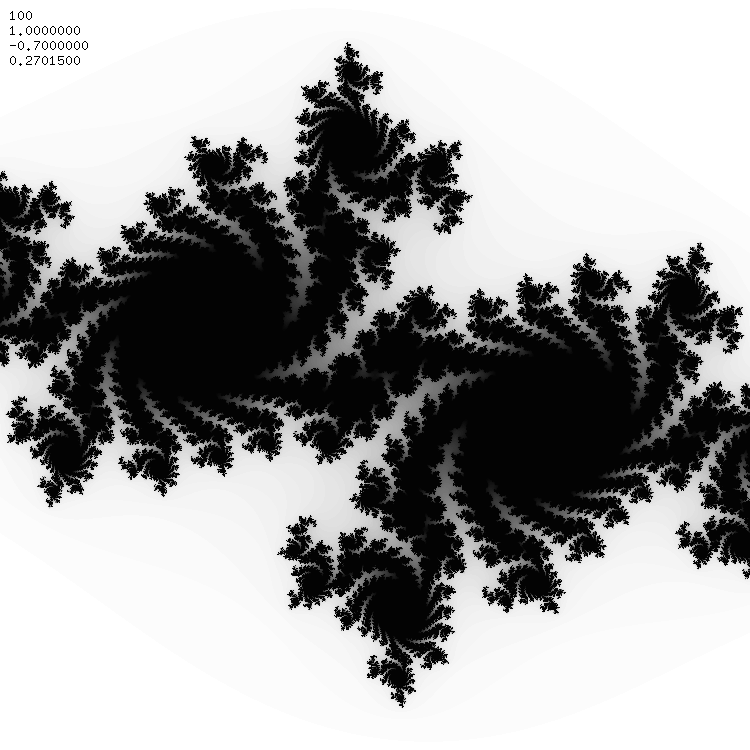
\includegraphics[width=0.2\textwidth]{images/Julia-Fractal.png}
%   \caption{Exampelimage}
% \end{figure}
%
% \subparagraph{Unforgeability}
% \label{subp:subparagraph_name}
%
% Graphic by \url{http://en.wikipedia.org/wiki/Pretty_Good_Privacy#/media/File:PGP_diagram.svg
